%
% This is the LaTeX template file for lecture notes for EE 382C/EE 361C.
%
% To familiarize yourself with this template, the body contains
% some examples of its use.  Look them over.  Then you can
% run LaTeX on this file.  After you have LaTeXed this file then
% you can look over the result either by printing it out with
% dvips or using xdvi.
%
% This template is based on the template for Prof. Sinclair's CS 270.

\documentclass[twoside]{article}
\usepackage{graphics}
\usepackage{amssymb}
\usepackage{pgfplots}
\usepackage{amsmath}
\pgfplotsset{width=7cm,compat=1.9}
\setlength{\oddsidemargin}{0.25 in}
\setlength{\evensidemargin}{-0.25 in}
\setlength{\topmargin}{-0.6 in}
\setlength{\textwidth}{6.5 in}
\setlength{\textheight}{8.5 in}
\setlength{\headsep}{0.75 in}
\setlength{\parindent}{0 in}
\setlength{\parskip}{0.1 in}

%
% The following commands set up the lecnum (lecture number)
% counter and make various numbering schemes work relative
% to the lecture number.
%
\newcounter{lecnum}
\renewcommand{\thepage}{\thelecnum-\arabic{page}}
\renewcommand{\thesection}{\thelecnum.\arabic{section}}
\renewcommand{\theequation}{\thelecnum.\arabic{equation}}
\renewcommand{\thefigure}{\thelecnum.\arabic{figure}}
\renewcommand{\thetable}{\thelecnum.\arabic{table}}
\newcommand{\longsquiggly}{\xymatrix@C=1.5em{{}\ar@{~>}[r]&{}}}

%
% The following macro is used to generate the header.
%
\newcommand{\lecture}[4]{
   \pagestyle{myheadings}
   \thispagestyle{plain}
   \newpage
   \setcounter{lecnum}{#1}
   \setcounter{page}{1}
   \noindent
   \begin{center}
   \framebox{
      \vbox{\vspace{2mm}
    \hbox to 6.28in { {\bf EE 382N: Distributed Systems
                        \hfill Fall 2017} }
       \vspace{4mm}
       \hbox to 6.28in { {\Large \hfill Lecture #1: #2  \hfill} }
       \vspace{2mm}
       \hbox to 6.28in { {\it Lecturer: #3 \hfill Scribe: #4} }
      \vspace{2mm}}
   }
   \end{center}
   \markboth{Lecture #1: #2}{Lecture #1: #2}
   %{\bf Disclaimer}: {\it These notes have not been subjected to the
   %usual scrutiny reserved for formal publications.  They may be distributed
   %outside this class only with the permission of the Instructor.}
   \vspace*{4mm}
}

%
% Convention for citations is authors' initials followed by the year.
% For example, to cite a paper by Leighton and Maggs you would type
% \cite{LM89}, and to cite a paper by Strassen you would type \cite{S69}.
% (To avoid bibliography problems, for now we redefine the \cite command.)
% Also commands that create a suitable format for the reference list.
\renewcommand{\cite}[1]{[#1]}
\def\beginrefs{\begin{list}%
        {[\arabic{equation}]}{\usecounter{equation}
         \setlength{\leftmargin}{2.0truecm}\setlength{\labelsep}{0.4truecm}%
         \setlength{\labelwidth}{1.6truecm}}}
\def\endrefs{\end{list}}
\def\bibentry#1{\item[\hbox{[#1]}]}

%Use this command for a figure; it puts a figure in wherever you want it.
%usage: \fig{NUMBER}{SPACE-IN-INCHES}{CAPTION}
\newcommand{\fig}[3]{
			\vspace{#2}
			\begin{center}
			Figure \thelecnum.#1:~#3
			\end{center}
	}
% Use these for theorems, lemmas, proofs, etc.
\newtheorem{theorem}{Theorem}[lecnum]
\newtheorem{lemma}[theorem]{Lemma}
\newtheorem{proposition}[theorem]{Proposition}
\newtheorem{claim}[theorem]{Claim}
\newtheorem{corollary}[theorem]{Corollary}
\newtheorem{definition}[theorem]{Definition}
\newenvironment{proof}{{\bf Proof:}}{\hfill\rule{2mm}{2mm}}

% **** IF YOU WANT TO DEFINE ADDITIONAL MACROS FOR YOURSELF, PUT THEM HERE:

\begin{document}
%FILL IN THE RIGHT INFO.
%\lecture{**LECTURE-NUMBER**}{**DATE**}{**LECTURER**}{**SCRIBE**}
\lecture{1}{September 5}{Dr.Vijay Garg}{Shailesh Kelkar and Daniel Cabrera}
%\footnotetext{These notes are partially based on those of Nigel Mansell.}

% **** YOUR NOTES GO HERE:

% Some general latex examples and examples making use of the
% macros follow.  
%**** IN GENERAL, BE BRIEF. LONG SCRIBE NOTES, NO MATTER HOW WELL WRITTEN,
%**** ARE NEVER READ BY ANYBODY.
\section{Recap}
Happened-before relation ($\rightarrow$) is the smallest relation such that
\newline
1. if ($e \prec f$) in the same process, then (e$\rightarrow$f) where $\prec$ is locally precedes.
\newline
2. if ($e \rightsquigarrow f$), then (e$\rightarrow$f) where $\rightsquigarrow$ is remotely precedes.
\newline
3. if ($\exists g: $($e \rightarrow g$) $\land$ ($g \rightarrow f$)), then (e$\rightarrow$f).

Thus, 
$\rightarrow$ : $(\prec \cup \rightsquigarrow)^+$ where + is transitive closure.
\section{Topics}
\begin{enumerate}
\item Logical Clock
\item Physical Clock
\item Down-sets
\item Principal Ideals
\item Vector Clock
\item Dilworth's Theorem
\end{enumerate}

\section{Logical Clock}
\subsection{Definition}
A map C:E $\rightarrow \mathbb{N}$ is a logical clock if 
$\forall$ e,f $\in$ E: ($e \rightarrow f$) $\Rightarrow$ C(e) $<$ C(f).
In short, C is the function that preserves the structure.
\subsection{Logical Clock Algorithm}
The variable c (integer) is initialized to 0.
\newline
1. For internal events, c++ (increment c by 1).
\newline
2. For send event, c++ and piggyback c with message.
\newline
3. For receive event of message having logical value d, c := max(c,d) + 1.
\newline
{\tt Note:C(e)$<$C(f) does not imply that e$\rightarrow$f}
\newline
Consider, C(e) = 5 and C(f) = 7, we can only conclude that f did not happen before e. Two possibilities exist : e happened before or concurrent with f.

Sometimes, events need to have unique timestamps.In this case, (logical clock value, Process ID) becomes the timestamp. In case of a tie, event with smallest process id wins.
Example
\begin{center}
\includegraphics[width=3.0 in]{LogicalClock}\\
\end{center}

\section{Physical Clock}
\subsection{Terminology}
Let G = (V,E) be undirected graph representing topology.
\begin{center}
\begin{tikzpicture}
\begin{axis}[
    axis lines = left,
    xlabel = $t$,
    ylabel = {$C(t)$},
]
%Below the red line is defined
\addplot [
    domain=0:10, 
    samples=50, 
    color=blue,
]
{x};
\addlegendentry{ideal}
%Here the blue line is defined
\addplot [
    domain=0:10, 
    samples=50, 
    color=red,
    ]
    {2*x};
\addlegendentry{running fast}
\addplot [
    domain=0:10, 
    samples=50, 
    color=black,
    ]
    {0.5*x};
\addlegendentry{running slow}
\end{axis}
\end{tikzpicture}
\end{center}

Drift rate = $| 1 - \frac{dc}{dt}| < \kappa$
\newline
\newline
$\tau$ = Synchronization Period (Every $\tau$ units of time, send your clock value to all your neighboring nodes)
\subsection{Lamport's Physical Clock Algorithm}
1. Assume, every sent message takes time in [$\mu, \mu+\xi$] to reach destination.
\newline
2. On receiving a message timestamped with D, C:= max$(C, D+\mu)^+$ where + indicates that it is fractionally bigger (smallest level of granularity).
Still, there exists uncertainty in synchronization($\epsilon$)
\newline
$|C_{i}(t) - C_{j}(t)| < \epsilon$  
\newline
Diameter of the graph(d) = $max_{i,j}$ (length of the shortest path from i to j)
\newline

$\boxed{\epsilon \approx d(2\kappa\tau + \xi)}$
\newline

Advantage of physical clock is that is satisfies logic clock property. 

\section{Down Sets}
\subsection{Terminology}
Let (X,$\leqslant$) be any poset. We call a subset Y $\subseteq$ X a down-set if:\\

\centerline{(z $\in$ Y) $\land$ (y $\leqslant$ z)$\Rightarrow$ (y $\in$ Y).}

Example 1\\
\begin{center}
\includegraphics[width=3.0 in]{Downset}\\
\end{center}
Y = \{ D \} is not a downset.\\
Y = \{ C, A \} is a downset.\\
Example 2\\
\begin{center}
\includegraphics[width=3.0 in]{Downset2}\\
\end{center}
D[\, E ]\, = \{ A, D, E \}

\section{Principal Ideals}
It refers to an ideal in a poset P generated by a single element x of P, which is to say the set of all elements less than or equal to x in P.

\section{Vector clocks}
When using vector clocks, the time domain is represented by a set of n-dimensional non-negative integer vector. A process Pi maintains a vector $VT_{i}$[\,1...n]\, where $VT_{i}$[\,i]\, is the local logical clock of Pi and describes the logical time progress at the process Pi.\\

Process Pi uses the following two rules R1 and R2 to update its clock:


\begin{itemize}
\item R1: Before executing an event, process Pi, updates its local logical time:\\
\centerline{$VT_{i}$[\,i]\, = $VT_{i}$[\,i ]\, + d where d  $>$ 0}\\
\item R2: Each message m is piggybacked with the vector VT of the sender process at sending time. On the receipt of such a message (m,vt), process Pi executes the following actions:
\begin{enumerate}
\item Update its global logical time as follows:\\
\centerline{1 $\leq$ K $\leq$ n : $VT_{i}$[\,i]\, := max($VT_{i}$[\,k]\,, VT[\,k]\,) }
\item Execute R1
\item Deliver the message m

\end{enumerate}




\end{itemize}
\newpage
Example
\begin{center}
\includegraphics[width=3.0 in]{VectorClocks}\\
\end{center}

\section{Dilworth's Theorem(1950's)}
\subsection{Theorem}
Any poset can be decomposed into w chains where w is the width of the poset. This is necessary and sufficient condition.
\subsection{Proof}
The basic idea is that when new element x comes up, we have to show that we can add it to one of the existing w chains.
\newline
\tt(To be continued...) 

\section*{References}
\beginrefs
\bibentry{ACM78}{\sc Leslie, Lamport},
Time, clocks, and the ordering of events in a distributed system,
{\it Communications of the ACM\/}~{\bf 21} (1978),
pp.~558--565.
\bibentry{Cambridge}{\sc Kshemkalyani, Ajay},
Distributed Computing: Principals, algorithms, and systems (2008)
\endrefs
\end{document}


